\subsection{\label{sec:radio}The Radio Lightcurve}
Minimal cloud cover and no sustained winds on the day of the eclipse contributed to a nearly issue free radio lightcurve.
We addressed 3 sources of error in our project: A strong gust of wind pushed the telescope off target for a few seconds, an issue with the accuracy of our polar alignment, causing the telescope to be slightly off target by the end of observation, and local sources of interference.
In order for this raw data to be compared to the optical lightcurve, these errors must be addressed.
A number of data analysis methods were used to do this:
\paragraph{Linear Adjustment function}
The first step in our data analysis is to correct for the tracking error.
We found average Analog to Digital Unit (ADU) counts for the duration of time after 4th contact and average ADU counts for the same duration of time before 1st contact.
We then created a linear function that shifts the data at the end of the lightcurve upward and decreases in effect to 0 at 1st contact.
\paragraph{Smoothing}
The next step is to smooth the data.
Our choice to smooth the data came from the need to reduce noise/random spikes in the data to get a better idea of the shape of the curve.
We chose to apply a Savitzky-Golay\cite{savitzky_golay_1964} filter to do this, which smoothes the data and removes noise.
\paragraph{Normalization}
The final step is to normalize the data.
Normalization is the process by which the data of a graph is scaled by a constant such that the highest points are equal to 100, essentially making the data a percentage of its highest value.
This is done after smoothing to avoid issues with noise spikes.
Converting the ADU counts to a relative brightness makes it possible to compare with the optical lightcurves.
\\
Now that the raw data has been refined, a neat radio lightcurve of the eclipse remains.
\subsection{\label{sec:optical}The Optical Lightcurve}
We collected optical lightcurve data to compare contact times, the depth of the eclipse, and the shape of the lightcurve to our radio observations. Our two sources include a livestream lightcurve using a solar filter-equipped optical telescope, and a Vernier Light Sensor (LS-BTA) pointed straight up at the sky.
\paragraph{The Livestream Lightcurve}
The livestream lightcurve was created by grayscaling the image of the eclipse and using Otsu thresholding to only count pixels above a certain value.
To get the time for each data point, we took an image of the in-video clock at the same time we counted the pixels of the eclipse and used computer vision to recognise the characters in the clock, giving us the time at which the frame was pixel-counted.
The number of pixels of the solar disk over time can then be normalized to a relative brightness.
We compared this livestream lightcurve to a theoretical lightcurve generated by the software \texttt{Stellarium}\cite{zotti_simulated_2020}, and were happy to see that the livestream and theoretical lightcurves overlap quite well.
\paragraph{The Light Sensor Lightcurve}
The light sensor used to collect data during the solar eclipse was the Vernier Light Sensor (LS-BTA) pointed at the sky.
Dr. Todd Abel and Shane Ayotte provided the light sensor data, which we normalized to relative brightness.
Because the light sensor data had timestamps included, we used it to confirm the accuracy of our other lightcurves timings.
\\
By stacking the lightcurves, we observed that all three had a very similar shape, with heavy overlap between the theoretical and livestream lightcurves.
This implies that our lightcurves are accurate and can be used to compare with our radio lightcurve to determine the size of the sun’s radio emission.
\\
\begin{figure}
    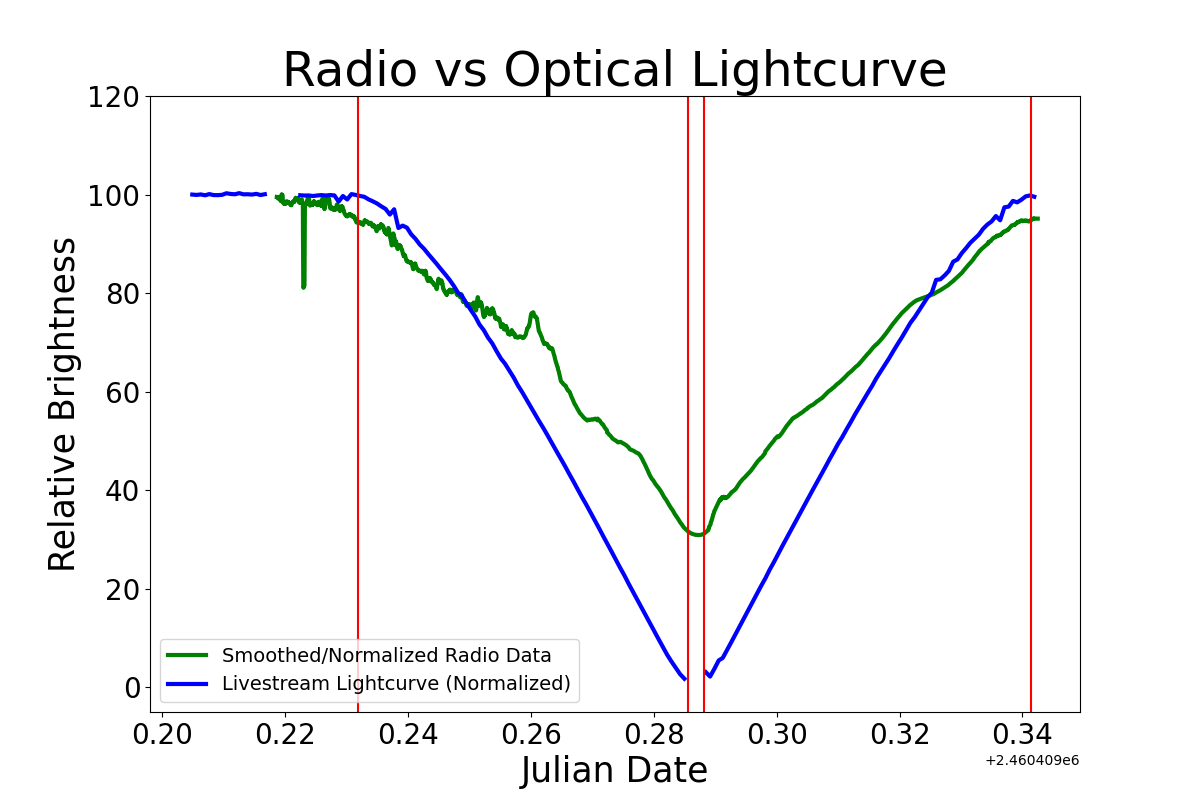
\includegraphics[width=0.5\textwidth]{figures/radioOpticalComparison}
    \caption{\label{fig:radioOpticalComparison} A comparison of the smoothed/normalized radio lightcurve and the normalized optical lightcurve generated from the livestream.}
\end{figure}